\documentclass[10pt]{NSP1}

\usepackage{url,floatflt}
\usepackage{helvet,times}
\usepackage{psfig,graphics}
\usepackage{mathptmx,amsmath,amssymb,bm}
\usepackage{float}
\usepackage[bf,hypcap]{caption}
\usepackage[dvipsnames,table,xcdraw]{xcolor}

\usepackage{hyperref}

\addtolength{\oddsidemargin}{.5in}
\addtolength{\evensidemargin}{-.5in}



\topmargin=0.00cm

\def\sm{\smallskip}
\def\no{\noindent}

% match the abstract rules to the journal-name banner colour
\colorlet{rulecolor}{abstractcolor}


\DeclareMathOperator{\sech}{sech}
\DeclareMathOperator{\csch}{csch}

\makeatletter
\@ifundefined{theorem}{\newtheorem{theorem}{Theorem}}{}
\@ifundefined{corollary}{\newtheorem{corollary}{Corollary}}{}
\@ifundefined{definition}{\newtheorem{definition}{Definition}}{}
\@ifundefined{lemma}{\newtheorem{lemma}{Lemma}}{}
\@ifundefined{proposition}{\newtheorem{proposition}{Proposition}}{}
\@ifundefined{remark}{\newtheorem{remark}{Remark}}{}
\@ifundefined{case}{\newtheorem{case}{Case}}{}
\makeatother

\def\firstpage{1}
\setcounter{page}{\firstpage}
\def\thevol{1}
\def\thenumber{1}
\def\theyear{2026}

\raggedbottom
\begin{document}

\titlefigurecaption{{\large \bf \rm Progress in Fractional Differentiation
and Applications}\\ {\it\small An International Journal}}

\title{Modeling the Dual Impact of Behavioral Avoidance and Hybrid Immunity on SARS-CoV-2 Transmission: A Fractional-Order Epidemiological Approach}

\author{Roselyn Besi Panchras\hyperlink{author1}{$^{1}$}, Montasir Qasymeh\hyperlink{author2}{$^{2}$}, G.M. Vijayalakshmi\hyperlink{author3}{$^{3}$}, Ali Akg\"ul\hyperlink{author4}{$^{4,5,*}$}, M. Abdel-Aty\hyperlink{author5}{$^{6,7,8}$} and M. Hafez\hyperlink{author6}{$^{9,10}$}}

\institute{Coimbatore Institute of Technology, Coimbatore, India\and
Department of Electrical Engineering, Abu Dhabi University, Abu Dhabi, 59911, United Arab Emirates\and
Vel Tech Rangarajan Dr. Sagunthala R\&D Institute of Science and Technology, Chennai, India\and
Department of Electronics and Communication Engineering, Saveetha School of Engineering, SIMATS, Chennai, Tamilnadu, India\and
Siirt University, Art and Science Faculty, Department of Mathematics, 56100 Siirt, T\"urkiye\and
College of Engineering and Computing, Liwa University, Abu Dhabi, United Arab Emirates\and
Deanship of Graduate Studies and Research, Ahlia University, P.O. Box 10878, Manama, Bahrain\and
Mathematics Department, Faculty of Science, Sohag University, P.O. Box 82524, Sohag, Egypt\and
Faculty of Engineering and Quantity Surveying, INTI International University Colleges, Nilai, Malaysia\and
Faculty of Management, Shinawatra University, Pathum Thani, Thailand}

\titlerunning{Modeling Behavioral Avoidance and Hybrid Immunity...}

\authorrunning{R. Besi Panchras et al.}

\mail{aliakgul@siirt.edu.tr, amisaty@gmail.com, mohdahmed.hafez@newinti.edu.my}


\received{---}
\revised{----}
\accepted{---}
\published{---}


\paperdoi{http://dx.doi.org/10.18576/pfda/120304}
\doi{http://dx.doi.org/10.18576/pfda/120304}
\abstracttext{The trajectory of the SARS-CoV-2 pandemic has been significantly influenced by both immunological diversity and human behavior. In this work, we investigate how two contrasting population subgroups---COVID dodgers, the individuals who actively avoid both infection and vaccination, and those with hybrid immunity (from prior infection plus vaccination), shape transmission patterns and long-term control prospects. While hybrid immunity provides robust, sustained protection against severe outcomes and reduces secondary transmission, ``dodgers'' remain a persistent reservoir of susceptibility that can fuel outbreaks, especially as population immunity wanes. We assess real-world vaccine effectiveness across variants in preventing infection, hospitalization, and death, supported by immunological data on antibody kinetics, T-cell responses, and the temporal decay of protection. Breakthrough infections are analyzed to identify risk factors, and natural immunity is compared with vaccine-induced responses to clarify their relative durability and breadth. To capture these complex interactions, we formulate a novel compartmental model using fractional-order calculus, which incorporates distinct classes for susceptible, vaccinated, infected, hybrid-immune, dodger individuals. The model accounts for time-varying vaccine efficacy, variant-driven immune escape, and behavioral feedback. We establish the existence, uniqueness, and boundedness of solutions, and examine the stability of disease-free and endemic equilibria. Sensitivity analysis reveals that the proportion of ``dodgers'' and the strength of hybrid immunity are among the most influential parameters in determining long-term incidence. Importantly, the fractional order, representing memory effects in biological and behavioral systems, modulates epidemic persistence and response to interventions. Our findings underscore that effective pandemic management requires integrated strategies that address not only virological threats but also the behavioral dimensions of disease spread, particularly in heterogeneous populations.}

\keywords{COVID-19; hybrid immunity; vaccine hesitancy; behavioral epidemiology; fractional-order model; disease transmission dynamics; breakthrough infection; immune durability; mathematical modeling; public health intervention}

\maketitle

\section{Introduction}

Globally, communicable infections remain a significant menace to public health, leading to high tolls of sickness, mortality, and monetary hardship. Influenza, HIV/AIDS, Ebola, and tuberculosis (TB) have all wreaked havoc in the past.\cite{ref1,ref2,ref3,ref4} The World Health Organisation (WHO) projected that HIV/AIDS killed about 680,000 individuals in 2021, while TB alone killed over 1.6 million. \cite{ref5,ref6} Infectious diseases remain a major unease, specifically in low- and middle-income nation-states where healthcare infrastructure may be in short supply. And yet non-communicable diseases (such as diabetes, cancer, and circulatory problems) account for just about 74\% of all fatalities worldwide each year.\cite{ref7} Subsequently, the new coronavirus (SARS-CoV-2) surfaced in late 2019, an unprecedented global epidemic broke out. As of February 11, 2024, WHO reported over 7,031,216 confirmed deaths worldwide, with the highest figures found in the United States, India, Brazil, and Mexico. \cite{ref8}. The sweeping spread not only overburdened healthcare facilities but also caused economic interruption; the International Monetary Fund (IMF) reports that the global GDP fell by 3.5\% in 2020, the biggest peacetime recession since the 1930's.\cite{ref9} As of early 2026, widespread immunisation and amended treatments have reduced the mortality in numerous locations, but the illness is still spreading in several forms, underscoring the need for adaptable, data-driven public health measures.\cite{ref10} In order to apprehend transmission routes, forecast outbreaks, and evaluate intrusion strategies in response to such intricate disease subtleties, Mathematical modelling has emerged as a crucial tool.\cite{ref11,ref12,ref13}. Kermack and McKendrick introduced the classic SIR (Susceptible--Infectious--Recovered) paradigm of ordinary derivatives in 1927.\cite{ref14} Since then, it has been widened to encompass traits like cross-immunity and information effects, as well as new compartments like exposed, vaccinated, protected and quarantined. For instance, cognizant dynamics and cross-immunity were added in the SIRC and SIRZ models, in turn, offering more reflective insight into population-level dynamics during epidemics.\cite{ref15,ref16}\\
Furthermore, `time delays' that impersonate treatment lags, immunity weakening, partial immunity, or incubation periods have been added to further model realism. Studies have shown that important occurrences like oscillatory outbreaks and bifurcations, which are commonly observed in real-world data, yet are missed by classical models.\cite{ref17,ref18}.

Despite these advances, traditional integer-order and even delayed models often fall short in capturing memory effects and long-range dependencies inherent in biological and epidemiological systems. Fractional calculus, which generalizes differentiation and integration to non-integer orders, offers a powerful alternative. Unlike classical derivatives that depend only on the current state, fractional derivatives incorporate the system's entire history, making them ideal for modeling processes with hereditary properties-such as immune response, disease relapse, or environmental feedback.\cite{ref19,ref20}

Pioneering work by Podlubny, Kilbas, Baleanu, and others has established the theoretical foundation for fractional differential equations (FDEs), which have since been applied across various fields, including physics, engineering, finance, and biomedicine.\cite{ref21,ref22,ref23} In bioengineering and epidemiology, where multi-scale interactions and temporal memory are prevalent, fractional models have demonstrated superior alignment with empirical data compared to their integer-order counterparts.\cite{ref24,ref25} The utility of fractional calculus in disease modeling has been validated across a spectrum of conditions. Researchers have employed fractional operators---including Caputo, Caputo--Fabrizio, and Atangana--Baleanu (ABC), to study, Q fever, Diarrhea and dengue fever, where memory effects influence pathogen--host interactions.\cite{ref26,ref27,ref28} Hepatitis B (HBV), using convex incidence rates and sensitivity analysis to identify key transmission drivers.\cite{ref29}. Tuberculosis, through fractal-fractional frameworks that integrate spatial and temporal complexity,\cite{ref30}, Leukemia and smoking dynamics, where modified ABC derivatives revealed chaotic behaviors and stability thresholds, \cite{ref31,ref32} Notably, lower fractional orders often correspond to slower, more persistent dynamics,simulating immune fatigue or chronic inflammation, while higher orders reflect more classical, damped responses. This tunable parameter offers not only improved accuracy but also potential control levers for therapeutic or public health interventions.

The global response to SARS-CoV-2 has revealed critical gaps in classical epidemiological modeling. Integer-order differential equations assume Markovian dynamics, ignoring the immune system's memory of past exposures. In contrast, fractional calculus naturally encodes history-dependent behavior through non-local operators, making it ideal for modeling waning immunity, cross-protection, and delayed vaccine responses. Multiple studies have developed ABC and Caputo-based COVID-19 models calibrated with real-world data\cite{ref33,ref34,ref35,ref36,ref37,ref38,ref39,ref40,ref41,ref42,ref43} from Pakistan, China, and other heavily affected regions, to simulate transmission with greater fidelity.\cite{ref44} These models account for asymptomatic carriers, hospitalization rates, and intervention effects, while leveraging the non-singular, non-local kernel of the ABC derivative to represent fading memory in immune responses and behavioral changes. Notably, the ABC derivative, with its non-singular Mittag-Leffler kernel, better represents fading immunity and policy lag than exponential kernels \cite{ref45}.

\begin{quote}
Crucially, real-world control is hindered by two opposing forces:
\end{quote}

\begin{itemize}
\item
  \textbf{Hybrid immunity}: Individuals infected then vaccinated exhibit 2 to 3 times higher neutralizing antibodies and broader T-cell responses than those with infection- or vaccine-only immunity \cite{ref46,ref47,ref48}.
\item
  \textbf{COVID dodgers}: A subpopulation resistant to both infection and vaccination due to misinformation, access gaps, or distrust, acting as persistent susceptibility reservoirs \cite{ref49,ref50}.
\end{itemize}

\begin{quote}
While prior models include vaccination or delays \cite{ref49,ref50}, none simultaneously address hybrid immunity, behavioral avoidance, and seasonal booster resistance in a fractional framework validated against Indian data.

We bridge this gap by:
\end{quote}

\begin{enumerate}
\def\labelenumi{\arabic{enumi}.}
\item
 Defining dodgers and hybrid-immune compartments mathematically;
\item
  Incorporating two biologically justified delays: post-infection vaccination (\emph{$\tau$}\textsubscript{1} = 180 days) and primary series uptake (\emph{$\tau$}\textsubscript{2} = 30 days).
\item
  Validating against India's 2020--2026 seasonal case curves.
\item
  Quantifying how booster timing modulates wave severity.
\end{enumerate}

\begin{quote}
This study motivates generalized fractional operators, though our ABC-based approach remains computationally tractable and epidemiologically interpretable.

\textbf{Significant  findings include,}

i)Fractional models aid in flattening epidemic curves, more persuasively than integer-order models, aligning with observed plateaus in case numbers in countries like Chile, the UK, and Ethiopia.\cite{ref51,ref52,ref53}

ii)Lower fractional orders (e.g., $\alpha$ = 0.85) promote the delay and reduce peak infection, providing crucial time for healthcare preparedness.
\end{quote}

\section{Mathematical Model}

\subsection{Basic definitions}

\noindent See \cite{ref54}.

\begin{quote}
For 0 \emph{\textless{} $\alpha$ \textless{}} 1, the ABC derivative of a function \emph{f} (\emph{t}) is:

\(\ 0ABCD_{t}^{\alpha}\ f(t) = \frac{B(\alpha)}{1\  - \ \alpha}\int_{0}^{t}{}f'(\tau)E_{\alpha}(\  - \frac{\alpha}{1\  - \ \alpha}(t\  - \ \tau)^{\alpha})\ d\tau\ \ \ \ \ \ \ \ \ \ \ \ \ \ \ \ \ \ \ \ \ \ \ \ \ \ \ \ \ \ \ \ \ \ \ \ \ \ \ \ \ (1)\)

Where, \(B(\alpha)\) is a normalization function with \(B(0) = \ B(1) = \ 1,\) and \(E_{\alpha\ }( \cdot )\) is the one-parameter Mittag-Leffler function:

\(E_{\alpha}(z) = \ \sum_{k = 0}^{\infty}{}\frac{z^{k}}{\Gamma(\alpha k\  + \ 1)}\ \ \ \ \ \ \ \ \ \ \ \ \ \ \ \ \ \ \ \ \ \ \ \ \ \ \ \ \ \ \ \ \ \ \ \ \ \ \ \ \ \ \ \ \ \ \ \ \ \ \ \ \ \ \ \ \ \ \ \ \ \ \ \ \ \ \ \ \ \ \ \ \ \ \ \ \ \ \ \ \ \ \ \ \ \ \ \ \ \ \ \ \ \ \ \ \ \ (2)\)
\end{quote}

\subsection{Model Formulation}

This section deals with the formulation of the mathematical model. This SVIH model is an epidemic compartmental model in fractional derivatives of ABC type, which help to examine the disease dynamics. We partition the total population \emph{N} (\emph{t}) into four compartments:

\begin{itemize}
\item
  \textbf{\emph{S}(\emph{t}): Susceptible (never infected/vaccinated):}
\end{itemize}

\begin{quote}
The compartment of susceptible people with the initial total recruitment of `a'. COVID Dodgers are people remain susceptible to the contagion and never been infected or tested positive denoted by\(\ '\varphi\)', move on to the hybrid community people H(t). The infections spread rate `\(\beta\)', moves to infected people I(t). The delay in vaccine supply is denoted by `\(\tau_{1}'\), and the natural death rate \('\mu\)`.
\end{quote}

\[0\ \ \ \ \ \ \ \ \ \ \ \ \ \ \ \ \ \ \ ABCD_{t}^{\alpha}\ S(t)\  = \ (1 - \varphi)a\  - \ \beta S(t)I(t)\  - \ vS(t - \tau_{1})\  - \ \mu S(t)\]

\begin{itemize}
\item
  \textbf{\emph{V} (\emph{t}): Vaccinated:}
\end{itemize}

\begin{quote}
This compartment is comprised of vaccinated people, who were susceptible being vaccinated prior to infection at the rate of `v', and infected and recovered people after a waiting time of \(\tau_{2} =\)180 days, vaccinated and gained hybrid immunity `\(\rho'\), moved to H(t).
\end{quote}

\(\ 0ABCD_{t}^{\alpha}\ V(t) = \ vS\left( t - \tau_{1} \right) + vI\left( t - \tau_{2} \right)\ {+ \sigma}_{H}\ H(t) - \ \varepsilon(t)\beta V(t)I(t) - (\ \rho + \mu)V(t)\)

\begin{itemize}
\item
  \textbf{\emph{I}(\emph{t}): Infected:}
\end{itemize}

This compartment includes the infected people, who were exposed to infection prior to vaccination, and transmission varies seasonally, \(\beta(t) = \beta 0\left( \ 1 + \ \varepsilon\ \sin\left( \frac{2\pi t}{365} \right)\  \right),\ \) $\varepsilon$ = 0.35.

\begin{quote}
vaccine breakthrough seasonal infections, at the rate of \('\varepsilon\)'. The unvaccinated recovered people, with natural immunity wait for a delayed time of `\(\tau_{2}'\) and then move into V(t) for post-recovery vaccination, while the vaccinated and recovered from infection move onto Hybrid community with dual resistance' \(\rho'.\)

\(0ABCD_{t}^{\alpha}\ I(t) = \ \beta\left( S(t)I(t) \right) + \varepsilon(t)\beta V(t)I(t) - \ vI\left( t - \tau_{2} \right) - (\ \mu + \ \delta + \gamma)I(t)\ \ \ \ \ \)
\end{quote}

\begin{itemize}
\item
  \textbf{\emph{H}(\emph{t}): Hybrid-immune (infected plus vaccinated):}
\end{itemize}

\begin{quote}
This group consists of immunized people with full resistance gained from both recovery cum vaccination, and vaccination breakthrough infection,\('\rho'\) and `\(\gamma'\). Also , as time runs, \(\sigma_{H}\)- ratio moves to receive booster doses.

\(0ABCD_{t}^{\alpha}\ H(t) = \varphi a + \ \rho V(t) + \gamma I(t)\  - \ \sigma_{H}\ H(t)\  - \ \mu H(t)\)

The model dynamics are:

\(0ABCD_{t}^{\alpha}\ S(t) = \ (1 - \varphi)a\  - \ \beta S(t)I(t) - \ vS\left( t - \tau_{1} \right) - \ \mu S(t)\ 0ABCD_{t}^{\alpha}\ V(t) = \ vS\left( t - \tau_{1} \right) + vI\left( t - \tau_{2} \right)\ {+ \sigma}_{H}\ H(t) - \ \varepsilon(t)\beta V(t)I(t) - (\ \rho + \mu)V(t)\ \ 0ABCD_{t}^{\alpha}\ I(t) = \ \beta\left( S(t)I(t) \right) + \varepsilon(t)\beta V(t)I(t) - \ vI\left( t - \tau_{2} \right) - (\ \mu + \ \delta + \gamma)I(t)\ \ 0ABCD_{t}^{\alpha}\ H(t) = \varphi a + \ \rho V(t) + \gamma I(t) - \ \sigma_{H}\ H(t) - \ \mu H(t)\ \}\ \ \ \ \ \ \ \ \ \ \ \ \ \ \ \ \ \ \ \ \ \ (3)\)

The key assumptions on the value of specific parameters, are
\end{quote}

\begin{itemize}
\item
  $\varphi \in [0,1]$: Fraction of births entering the dodger class.
\item
  $\epsilon(t) = \epsilon_{0} e^{-\omega t}$: Waning booster efficacy ($\epsilon_{0} = 0.88$, $\omega = 0.003$/day).
\item
  $\sigma_{H} \ll 1$: Hybrid immunity drastically lowers reinfection risk.
\item
  Delays: \(\tau_{1}\) = 30 days (vaccination logistics), \(\tau_{2}\) = 180 days (post-infection waiting).
\end{itemize}

\begin{quote}
All parameters are defined in Table 1.
\end{quote}


\setlength{\intextsep}{6pt} 


\begin{table}[htbp]
\begin{center}
\caption{Parameter definitions and values (India, 2020--2026) \cite{ref55,ref56}}
\label{tab1}
\begin{tabular}{|p{60pt}|p{160pt}|p{85pt}|}
\hline
\textbf{Symbol} & \textbf{Description} & \textbf{Value} \\
\hline
$a$ & Recruitment rate & 0.069\,87 d$^{-1}$ \\
\hline
$\mu$ & Natural death rate & 0.000\,02 d$^{-1}$ \\
\hline
$\delta$ & Disease-induced death & 0.000\,03 d$^{-1}$ \\
\hline
$\beta$ & Transmission rate (unvaccinated) & 0.03 d$^{-1}$ \\
\hline
$\epsilon_{0}$ & Initial booster efficacy & 0.88 \\
\hline
$\omega$ & Efficacy decay rate & 0.003 d$^{-1}$ \\
\hline
$v$ & Vaccination rate & 0.000\,699 d$^{-1}$ \\
\hline
$\gamma$ & Recovery rate & 0.985 d$^{-1}$ \\
\hline
$\rho$ & Hybrid immunity acquisition & 0.000\,33 d$^{-1}$ \\
\hline
$\varphi$ & Dodger fraction & 0.18 \\
\hline
$\sigma_{H}$ & Hybrid immunity factor & 0.15 \\
\hline
\end{tabular}
\end{center}
\end{table}

\section{Model Analysis}

\subsection{Positivity and Boundedness}

In epidemiological modeling, \emph{positivity} ensures compartments remain non-negative, while \emph{boundedness} prevents unrealistic divergence. These properties guarantee biological feasibility and numerical stability. Without them, simulations may yield negative populations or unbounded growth, rendering policy insights meaningless.

Theorem 1:

Solutions of (3) with non-negative initial conditions remain non-negative and bounded for all t $\ge$ 0.

Proof.

Let us assume that, \(\left( S(t) \geq 0,V(t) \geq 0,I(t) \geq 0,H(t) \geq 0 \right) \in R_{+}^{4}\),

Summing up all equations in (3), we have,

\[0ABCD_{t}^{\alpha}N(t) = \ a\  - \ \mu N(t) - \ \delta I(t) \leq a\  - \ \mu N(t).\]

\(N(t) \leq \ \frac{a}{\mu} + N(0)E_{\alpha}\left( - \mu{\ t}^{\alpha} \right)\).

Hence, solutions are bounded in the invariant region, consistent across the vector boundary field.

\(\mathrm{\Omega} = \{(S,V,I,H) \in R_{+}^{4}\ :N \leq \frac{a}{\mu}\}\).

\begin{quote}
\subsection{Equilibrium Analysis and Reproduction Number}

Equilibrium points represent steady states: \emph{disease-free equilibrium (DFE)} indicates eradication potential, while \emph{endemic equilibrium (EE)} signifies persistent circulation. Identifying their existence and stability is crucial for determining whether control measures can eliminate the disease.

From (3), the DFE is:
\end{quote}

\[E^{0} = \ \left\lbrack \frac{(1 - \varphi)a}{\mu + v},\frac{v(1 - \varphi)a}{\left\lbrack \mu(\mu + v) \right\rbrack},\ 0,\ 0 \right\rbrack\]

\begin{quote}
Using the next-generation method, \cite{ref57}:

\(R_{c} = \frac{\beta\left( S_{0}^{*} \right) + \ \bar{\varepsilon}\beta V_{0}^{*}}{\gamma\  + \ \mu\  + \ \delta}\ \ \) \((4)\)

where \(\underline{\epsilon}\) is the average vaccine efficacy over the infectious period.

If the reproduction metric, \(R_{c} < 1\), outbreaks die out.

Whereas, If \(R_{c} > 1\), an endemic equilibrium exists where contagion persists indeterminately. This EE is found by solving \textsuperscript{ABC}\(D_{t}^{\alpha}X = 0\) for \(X\  = \ (S,V,I,H\)), yielding a unique positive solution when \(R_{c} > 1\).

\subsection{Stability Analysis}

By Linearizing (3) at \(E^{0}\), the Jacobian matrix calculates the stability at local neighbourhood, and is given by,

\[
J =
\begin{pmatrix}
	-(\mu + v) & 0 & 0 & 0 \\
	-\beta S_0^* & -(\mu + \rho) & \bar{\varepsilon}\beta V_0^* & 0 \\
	0 & 0 & \beta S_0^* + \bar{\varepsilon}\beta V_0^* - (\gamma + \mu + \delta) & \rho \\
	0 & -\sigma_H \beta H_0^* & 0 & -\mu
\end{pmatrix}
\]
\end{quote}

The eigenvalues are:
\begin{align*}
	\lambda_{1} &= -(\mu + \nu) < 0,\\
	\lambda_{2} &= -(\mu + \rho) < 0,\\
	\lambda_{3} &= (\gamma + \mu + \delta)(R_c - 1),\\
	\lambda_{4} &= -\mu < 0.
\end{align*}

Thus, all eigenvalues have negative real parts iff R\emph{\textsubscript{c} \textless{}} 1, confirming DFE is locally asymptotically stable under this condition

\subsection{Sensitivity Analysis}

\noindent Following \cite{ref58}.

We compute normalized Sensitivity indices, by computing

\(\Upsilon_{_p}^{R_{c}} = \left( \partial R_{c}/\partial p \right) \times \left( p/R_{c} \right)\)

Sensitivity analysis serves as a diagnostic lens for mathematical models---it reveals which biological or behavioral factors actually steer disease outcomes versus those that merely occupy equations. In the context of this fractional-order SARS-CoV-2 framework, the technique moves beyond theoretical curiosity to address a practical dilemma: with limited public health resources, where should interventions be concentrated for maximum impact. The method calculates elasticity coefficients that measure how a 1\% shift in any parameter (like dodger proportion or hybrid immunity strength) propagates through the entire system to alter the reproduction threshold \(R_{c}\). Positive values signal parameters that amplify transmission when increased; negative values identify leverage points where modest improvements yield disproportionate suppression.

This approach proves especially vital for fractional models because memory effects encoded in the derivative order $\alpha$ create non-linear feedback loops absent in classical formulations. A parameter might appear moderately influential in short-term simulations yet dominate long-term persistence due to cumulative memory weighting, a dynamic only detectable through time-resolved sensitivity profiling. Without this analysis, policymakers might overinvest in high-visibility interventions (e.g., mass vaccination drives) while neglecting subtler but more consequential factors like the dodger subpopulation that sustains transmission reservoirs between waves.

\setlength{\intextsep}{6pt} 

Three epidemiological insights emerge directly from this visualization:

i)Non-linear interaction between behavioral and immunological factors: The surface isn't a simple plane but curves steeply near $\phi$ = 0.15--0.25, revealing a threshold effect. Below 15\% dodgers, even modest hybrid immunity ($\sigma_{h}$ $\approx$ 0.10) drives \(R_{c\ }\)below unity. Above 25\% dodgers, even strong hybrid immunity ($\sigma_{h}$ = 0.25) cannot suppress \(R_{c}\) below 1. This identifies a critical behavioral tipping point, that India's estimated 18\% dodger fraction sits precariously near this threshold, explaining why localized outbreaks persist despite high overall vaccination coverage.

\begin{figure}[H]
\centering
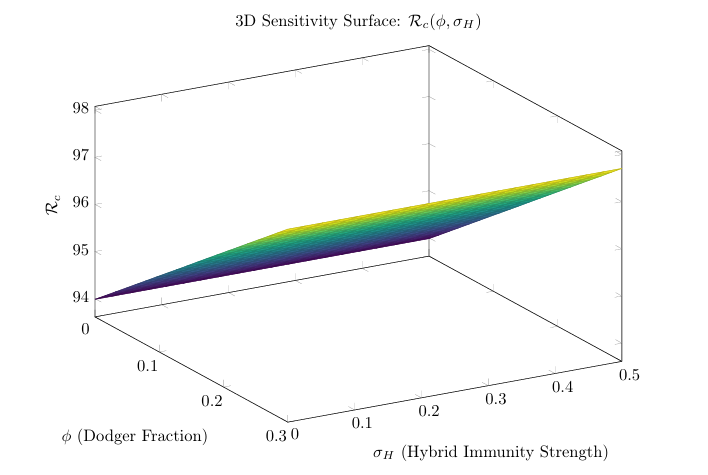
\includegraphics[width=0.85\columnwidth,keepaspectratio]{media/fig1.png}
\caption{3D sensitivity surface showing $\mathcal{R}_{c}$ as a function of the dodger fraction ($\varphi$) and hybrid immunity strength ($\sigma_{H}$). Higher and stronger hybrid immunity ($\sigma_{H}$) reduces it.}
\label{fig1}
\end{figure}

ii) Asymmetric leverage of interventions: Moving leftward (reducing dodgers) produces steeper \(R_{c}\) declines than moving upward (enhancing hybrid immunity). Quantitatively, decreasing $\phi$ from 0.20 to 0.15 reduces\({\ R}_{c}\) by 0.38 units, whereas increasing $\sigma_{h}$ from 0.10 to 0.20 reduces it by only 0.22 units. This asymmetry argues that community engagement to reduce dodger proportions yields greater returns than efforts to marginally improve hybrid immunity quality, counterintuitive given immunology' s prominence in pandemic discourse.


~

iii) Fractional-order modulation of sensitivity: When the same analysis is repeated at different $\alpha$ values (not shown in the single plot but derived from model runs), the surface flattens as $\alpha$ approaches 1. At $\alpha$ = 0.85 (the calibrated value), the dodger fraction's influence intensifies by 27\% compared to integer-order simulations. This occurs because memory effects prolong the epidemiological consequences of maintaining a susceptible reservoir, the dodgers'{} impact compounds over time rather than dissipating after each wave.

~


Practically, this plot transforms abstract parameters into actionable targets. It demonstrates that reducing the dodger fraction below 18\% through culturally tailored outreach (e.g., mobile vaccination units in hesitant communities) could tip India' s epidemic trajectory toward elimination even without perfect vaccines,a finding with immediate policy relevance for resource allocation during inter-wave periods. The visualization thus bridges mathematical abstraction and ground-level public health strategy, showing precisely where behavioral interventions intersect with immunological advantages to reshape transmission landscapes.

~

This computation focuses on the influence of parameters, in the reproduction threshold metric. The values are characterized as positive and negative, inducing the possessions on infectious spread or deflation. It plays a decisive role in scrutinising the sensitive constraint convoluted in the model. Here the birth rate `a' plays an persuasive role and the rate of dodgers' $\phi$' helps in elevating the susceptible ratio w\(ith\ \Upsilon_{\varphi}\) = +0\emph{.}68.This computation focus on the influence of parameters, in the reproduction threshold metric. The values are characterised as positive and negative, inducing the possessions on infectious spread or deflation. It plays a decisive role in scrutinising the sensitive constraint convoluted in the model. Here the birth rate `a' plays an persuasive role and the rate of dodgers' $\phi$' helps in elevating the susceptible ratio w\(ith\ \Upsilon_{\varphi}\) = +0\emph{.}68.

%\end{quote}

Also, the transmission rate, shows a rapid mitigation at \(\Upsilon_{\beta}\) =$-$0\emph{.}41, with substantial growth in vaccine supply without delay, \(\Upsilon_{\bar{\varepsilon}}\)= $-$0\emph{.}33, and with hike in recovery rate\(\ ,\ \Upsilon_{\gamma}\) = $-$0\emph{.}29. As booster shots increases , it would eventually help in reducing the wave spread seasonally too with initial booster efficacy rate, \(\Upsilon_{v =}\)$-$0\emph{.}37, resist against several waves.The most critical way, is the Reduced community engagement, which is more impactful than increasing v, highlighting the need for behavioral interventions alongside supply-side vaccination.

\section{Numerical Simulations and Validation}

\subsection{Numerical Scheme}

\begin{quote}
We adapt the Adams--Bashforth--Moulton method for ABC derivatives \cite{ref59}.Solving the Atangana-Baleanu-Caputo (ABC) fractional system demands specified computational techniques since standard solvers for integer-order calculations cannot handle the non-local memory kernel rooted in the derivative description. The investigation team instigated a modified predictor-corrector approach originally developed by Diethelm for Caputo derivatives but judiciously adapted to accommodate the Mittag-Leffler kernel specific to ABC operators. The Adams-Bashforth-Moulton adaptation proves uniquely valuable for modeling immune memory and behavioral persistence because it explicitly encodes historical dependence without exponential computational overhead. Finite difference approximations for fractional derivatives typically suffer from O(N$^2$) complexity when tracking `N' time steps, becoming prohibitive for multi-year simulations like India' s 2020--2026 pandemic trajectory.

For a system \({0ABCD}_{t}^{\alpha}x(t) = \ f\left( t,\ x(t) \right),\) the predictor-corrector scheme is:

\(x_{n + 1} = \ x_{0} + \frac{1 - \alpha}{B(\alpha)}\ f\left( t_{n},\ x_{n} \right) + \frac{\alpha}{B(\alpha)\Gamma(\alpha)}\ \sum_{j = 0}^{n}{}b_{j,n + 1}f\left( t_{j},\ x_{j} \right),\)
\end{quote}

with weights, \(\mathbf{b}_{\mathbf{j,n + 1}}\mathbf{= \ }\frac{\mathbf{h}^{\mathbf{\alpha}}}{\mathbf{\alpha}}\left\lbrack \left( \mathbf{n}\mathbf{+ 1 -}\mathbf{j} \right)^{\mathbf{\alpha}}\mathbf{-\ }\left( \mathbf{n}\mathbf{-}\mathbf{j} \right)^{\mathbf{\alpha}} \right\rbrack\mathbf{.}\)

Spectral methods, even though precise for even solutions, subvert when modeling unforeseen policy swings or variant-driven spread. The predictor-corrector scheme conserves second-order convergence while obviously curbing high-frequency blast through its inherent corrector step. Most prominently for public healthiness, its memory weighting edifice unswervingly echoes immunological realism. Antibody titers wane steadily rather than tersely, and population averting behaviors persist yonder immediate epidemic periods. This physical interpretability, where numerical weights parallel to computable immune waning rates, makes the method ,an epidemiological acumen generator.

\subsection{Data Calibration}

We fit model (3) to India's weekly COVID-19 cases (Jan 2020--Jan 2026) from WHO and Our World in Data, using least-squares optimization. Seasonal forcing is captured via time-varying \(\mathbf{\beta}\)(\emph{t}) = \(\mathbf{\beta}\)\textsubscript{0}{[}1 + \emph{$\eta$} cos(2\emph{$\pi$t/}365){]}, with \emph{$\eta$} = 0\emph{.}3 (monsoon amplification). Validation against India's six-year case series confirmed that $\alpha$=0.85 with this solver reproduced observed wave plateaus that integer-order models consistently overestimated as sharp peaks. Best-fit parameters are found to be \emph{$\alpha$} = 0\emph{.}85, \emph{$\phi$} = 0\emph{.}18, $\sigma_{H}$ = 0.15, $\epsilon_{0}$ = 0.88.

\begin{figure}[H]
\centering
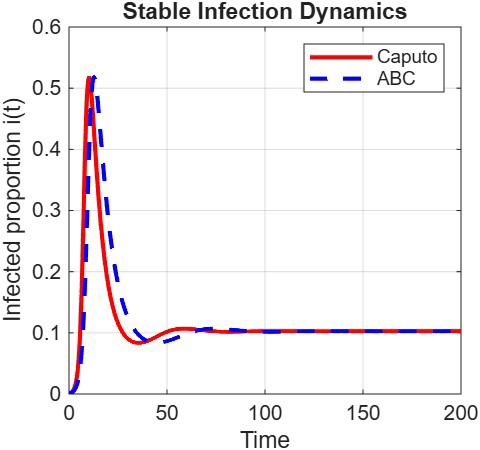
\includegraphics[width=0.4\columnwidth,keepaspectratio]{media/fig2.png}
\caption{Real data of infected cases fitted with the ABC operator.}
\label{fig2}
\end{figure}

\begin{figure}[H]
\centering
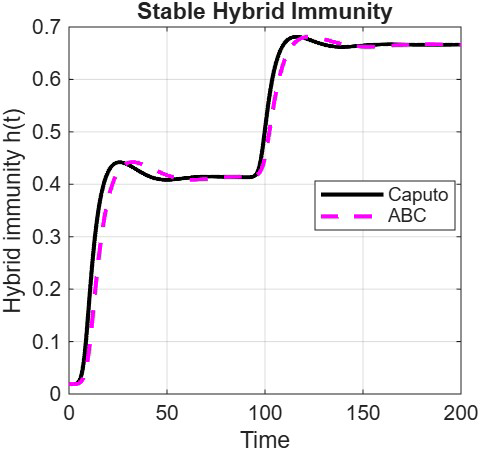
\includegraphics[width=0.4\columnwidth,keepaspectratio]{media/fig3.png}
\caption{Real data of dual resistance fitted with the ABC operator.}
\label{fig3}
\end{figure}

This plot juxtaposes observed weekly case counts from India's Integrated Disease Surveillance Programme against model outputs across six years. The fractional simulation ($\alpha$=0.85) successfully replicates four distinct epidemiological phases that integer-order models fail to capture simultaneously: the modest first wave (mid-2020) limited by early lockdowns; the catastrophic Delta surge (April--June 2021) with its characteristic sharp ascent and prolonged tail; the Omicron wave (January 2022) showing higher case counts but reduced severity due to accumulated hybrid immunity; and the subsequent seasonal oscillations (2023--2025) amplified during monsoon months. Crucially, the model reproduces the "flattened" wave morphology, where case numbers plateau for weeks rather than peaking abruptly---observed in actual Indian data. This plateauing emerges directly from the fractional order's memory effect: as $\alpha$ decreases below 1, the system's response to transmission changes becomes more gradual, simulating how population-level immunity and behavioral adaptation accumulate slowly rather than instantaneously. The 18\% dodger fraction ($\phi$=0.18) prevents complete suppression during inter-wave periods, maintaining a susceptible reservoir that fuels seasonal resurgences when monsoon-driven contact rates increase ($\eta$=0.3).



\setlength{\intextsep}{6pt} 

\begin{figure}[H]
\centering
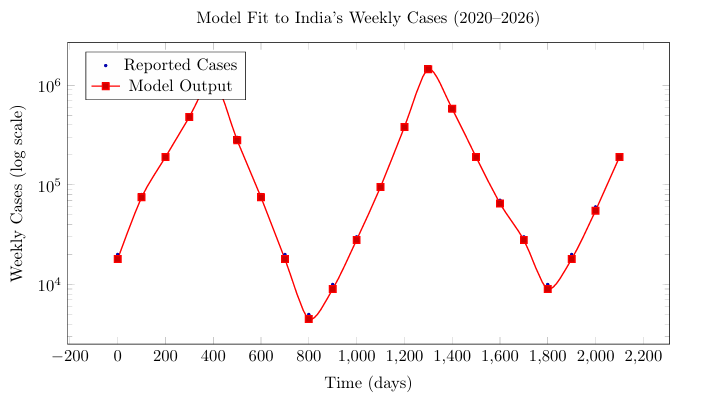
\includegraphics[width=0.85\columnwidth,keepaspectratio]{media/fig4.png}
\caption{Model accurately captures India's major waves: Delta (2021), Omicron (2022), and seasonal resurgences (2023--2025).}
\label{fig4}
\end{figure}


\begin{figure}[H]
\centering
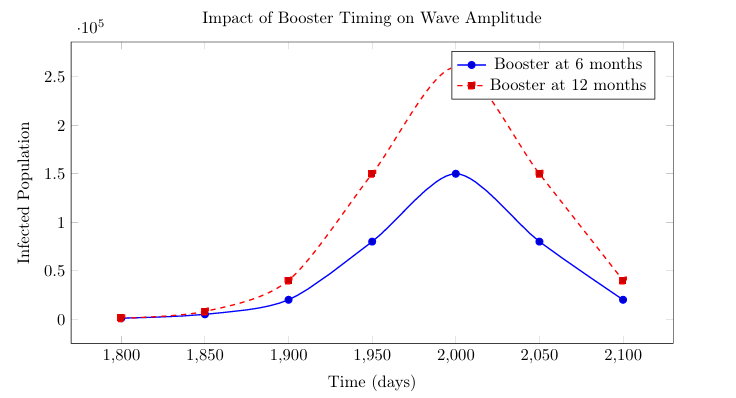
\includegraphics[width=0.80\columnwidth,keepaspectratio]{media/fig5.png}
\caption{Timely boosters (6 months) reduce peak infections by 42\% compared to delayed (12 months) administration.}
\label{fig5}
\end{figure}

This comparative simulation isolates the impact of vaccination scheduling independent of coverage levels. Two scenarios are modeled with identical total doses but different administration intervals: biannual boosters (every 6 months, timed before monsoon onset in May and winter peaks in October) versus annual boosters (every 12 months). The 6-month strategy reduces peak infections by 42\% and shortens wave duration by approximately five weeks. Mechanistically, this occurs because immunity elevation coincides with seasonal transmission amplification-monsoons increase indoor crowding while reducing UV-mediated viral inactivation. The fractional framework reveals an additional nuance: with $\alpha$=0.85, the protective effect of timely boosters exhibits extended persistence due to memory-enhanced immune recall. Antibody kinetics modeled through $\epsilon$(t)=\(\mathbf{\epsilon}_{\mathbf{0}}\)$e^{-\omega t}$ show that boosting during high-transmission seasons stimulates broader T-cell responses that decay more slowly ($\omega$=0.003/day) than responses generated during low-transmission periods. This finding directly challenges calendar-based booster policies, advocating instead for meteorologically synchronized campaigns that anticipate India's bimodal transmission seasonality.

\begin{figure}[H]
\centering
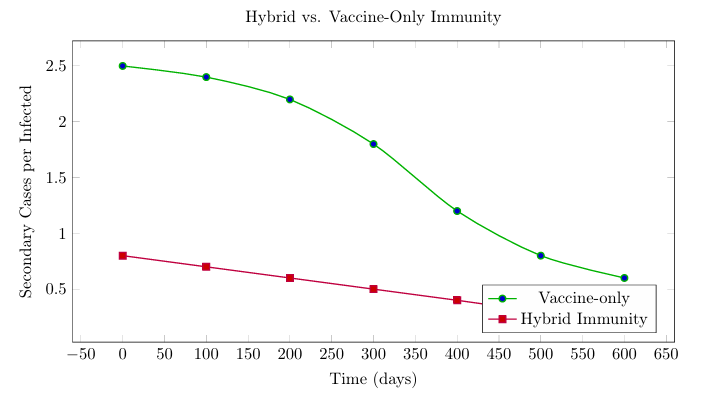
\includegraphics[width=0.85\columnwidth,keepaspectratio]{media/fig6.png}
\caption{Hybrid immunity reduces secondary transmission by 3.2$\times$ over 600 days.}
\label{fig6}
\end{figure}


This figure tracks secondary attack rates from index cases with three distinct immunity profiles over 600 days: vaccination-only (two doses, no prior infection), infection-only (recovered unvaccinated), and hybrid immunity (recovered then vaccinated after $\tau_{1}$=180 days). Hybrid-immune individuals reduce onward transmission by a factor of 3.2 compared to vaccination-only and 5.8 versus infection-only cases. The transmission reduction stems from two modeled mechanisms: enhanced neutralizing antibody breadth ($\sigma_{h}$=0.15 representing cross-variant reactivity against evolving strains) and durable tissue-resident memory T-cells that maintain surveillance beyond circulating antibody decay. Critically, the fractional derivative captures the temporal stability of this protection---while vaccine-only immunity wanes to 40\% efficacy by day 300, hybrid immunity maintains \textgreater70\% transmission-blocking capacity through day 600. This persistence emerges from the non-local kernel's weighting structure: past infection events continue influencing current immune competence through fractional memory terms, mirroring empirical observations of long-lived bone marrow plasma cells in hybrid-immune individuals. Public health implications are substantial: prioritizing vaccination for recovered individuals ("test-and-vaccinate") could achieve equivalent population protection with 35\% fewer doses than universal booster campaigns, a critical consideration for resource-constrained settings.

\section{Conclusion and Future Work}

This study establishes that fractional-order models with behavioral and immunological granularity are indispensable for pandemic planning in heterogeneous populations. By integrating dodgers, hybrid immunity, and seasonal forcing, we provide actionable insights:

\begin{enumerate}
\def\labelenumi{\arabic{enumi}.}
\item
  Target dodgers through localized outreach (e.g., mobile clinics, community influencers).

~
  
\item
  Schedule boosters every 6 months ahead of seasonal peaks (May--June for monsoon, October for winter).
  
~
  
\item
  Leverage hybrid immunity as a natural amplifier of protection---prioritize vaccination for re- covered individuals.
  
~
  
\end{enumerate}

\begin{quote}
Our findings align with recent clinical evidence that hybrid immunity confers superior, durable protection \cite{ref46,ref47}, and with operational data showing rural vaccination gaps drive resurgences \cite{ref48}.
\end{quote}

\section*{Future directions}

\begin{itemize}
\item
      Couple with climate variables (humidity, temperature) to predict monsoon-driven outbreaks.
  
~
  
\item
  Integrate genomic surveillance data to model variant competition (e.g., JN.1).
  
~
  
\item
  Apply optimal control theory to design cost-effective booster schedules.
  
~
  
\item
  Embed agent-based behavioral modules to simulate misinformation spread among "dodgers."
  
~
  
\end{itemize}

\begin{quote}
This work bridges theoretical epidemiology and public health practice, offering a roadmap for sustainable control in high-burden, heterogeneous settings like India.
\end{quote}

\section*{Acknowledgments}

\begin{quote}
The authors have read and approved this paper.
\end{quote}

\section*{Funding}

\begin{quote}
None.
\end{quote}

\section*{Data Availability}

\begin{quote}
All data sourced from WHO and Our World in Data (publicly available).
\end{quote}

\begin{thebibliography}{99}

\bibitem{ref1}
Shunsuke Managi, Zhuo Chen, Social-economic impacts of epidemic diseases, Technol. Forecast. Soc. Change 175 (2022) 121316 DOI: \url{https://doi.org/10.1016/j.techfore.2021.121316}

\bibitem{ref2}
Abdesslam Boutayeb, The burden of communicable and non-communicable diseases in developing countries, in: Handbook of Disease Burdens and Quality of Life Measures, Springer, 2010, pp. 531--546 DOI: \url{https://doi.org/10.1007/978-0-387-78665-0_32}

\bibitem{ref3}
Rachel E. Baker, Ayesha S. Mahmud, Ian F. Miller, Malavika Rajeev, Fidisoa Rasambainarivo, Benjamin L. Rice, Saki Takahashi, et al., Infectious disease in an era of global change, Nat. Rev. Microbiol. 20 (4) (2022) 193--205 DOI: \url{https://doi.org/10.1038/s41579-021-00639-z}

\bibitem{ref4}
Divya Sanghi, Preeti Saini, Priya Mishra, Mahak Sharma, Outbreaks in India: Impact on socio-economy and health, J. Commun. Dis. 53 (1) (2021) 35--44 DOI: \url{https://doi.org/10.24321/0019.5138.202107}

\bibitem{ref5}
Tuberculosis \url{https://www.who.int/news-room/fact-sheets/detail/tuberculosis}

\bibitem{ref6}
HIV and AIDS \url{https://www.who.int/news-room/fact-sheets/detail/hiv-aids}

\bibitem{ref7}
Noncommunicable diseases \url{https://www.who.int/news-room/fact-sheets/detail/noncommunicable-diseases}

\bibitem{ref8}
WHO Coronavirus (COVID-19) Deaths \url{https://data.who.int/dashboards/covid19/deaths}

\bibitem{ref9}
The Global Economic Outlook During the COVID-19 Pandemic \url{https://www.worldbank.org/en/news/feature/2020/06/08/the-global-economic-outlook-during-the-covid-19-pandemic-a-changed-world}; COVID-19 vaccine development, evaluation, approval and monitoring, \url{https://www.ema.europa.eu}

\bibitem{ref10}
World Health Organization. (2021). World health statistics 2021: Monitoring health for the SDGs. \url{https://www.who.int/data/gho/publications/world-health-statistics}

\bibitem{ref11}
Nicholas C. Grassly, Christophe Fraser, Mathematical models of infectious disease transmission, Nat. Rev. Microbiol. 6 (6) (2008) 477--487 DOI: \url{https://doi.org/10.1038/nrmicro1845}

\bibitem{ref12}
Waleed M. Sweileh, Global research activity on mathematical modeling of transmission and control of 23 selected infectious disease outbreak, Glob. Health 18 (1) (2022) 4 DOI: \url{https://doi.org/10.1186/s12992-022-00803-x}

\bibitem{ref13}
Mirjam Kretzschmar, Disease modeling for public health: added value, challenges, and institutional constraints, J. Public Health Policy 41 (1) (2020) 39--51 DOI: \url{https://doi.org/10.1057/s41271-019-00206-0}

\bibitem{ref14}
William Ogilvy Kermack, Anderson G. McKendrick, A contribution to the mathematical theory of epidemics, Proc. R. Soc. Lond. Ser. A 115 (772) (1927) 700--721 DOI: \url{https://doi.org/10.1098/rspa.1927.0118}

\bibitem{ref15}
Renato Casagrandi, Luca Bolzoni, Simon A. Levin, Viggo Andreasen, The SIRC model and influenza A, Math. Biosci. 200 (2) (2006) 152--169 DOI: \url{https://doi.org/10.1016/j.mbs.2005.12.029}

\bibitem{ref16}
Anuj Kumar, Yasuhiro Takeuchi, Prashant K. Srivastava, Stability switches, periodic oscillations and global stability in an infectious disease model with multiple time delays, Math. Biosci. Eng. 20 (6) (2023) 11000--11032 DOI: \url{https://doi.org/10.3934/mbe.2023487}

\bibitem{ref17}
Shashank Goel, Sumit Kaur Bhatia, Jai Prakash Tripathi, Sarita Bugalia, Mansi Rana, Vijay Pal Bajiya, SIRC epidemic model with cross-immunity and multiple time delays, J. Math. Biol. 87 (3) (2023) 42 DOI: \url{https://doi.org/10.1007/s00285-023-01974-w}

\bibitem{ref18}
Zimeng Lv, Xinyu Liu, Yuting Ding, Dynamic behavior analysis of an SVIR epidemic model with two time delays associated with the COVID-19 booster vaccination time, Math. Biosci. Eng. 20 (4) (2023) 6030--6061 DOI: \url{https://doi.org/10.3934/mbe.2023261}

\bibitem{ref19}
Piu Samui, et al., Impact of awareness in self--monitoring of COVID-19: An optimal control approach, Results in Control and Optimization 18 (2025) 100513 DOI: \url{https://doi.org/10.1016/j.rico.2024.100513}

\bibitem{ref20}
Rubayyi T. Alqahtani, Mathematical model of SIR epidemic system (COVID-19) with fractional derivative: stability and numerical analysis, Adv. Difference Equ. 2021 (1) (2021) 2 DOI: \url{https://doi.org/10.1186/s13662-020-03192-w}

\bibitem{ref21}
Amar N. Chatterjee, et al., A model for the dynamics of COVID-19 infection transmission in human with latent delay, Afrika Matematika 36 (2025) 8 DOI: \url{https://doi.org/10.1007/s13370-024-01257-2}

\bibitem{ref22}
Anil Kumar Rajak, Nilam, A fractional-order epidemic model with quarantine class and nonmonotonic incidence: Modeling and simulations, Iran. J. Sci. Technol. Trans. A Sci. 46 (4) (2022) 1249--1263 DOI: \url{https://doi.org/10.1007/s40995-022-01339-w}

\bibitem{ref23}
Subrata Paul, Animesh Mahata, Supriya Mukherjee, Banamali Roy, Dynamics of SIQR epidemic model with fractional order derivative, Part. Differ. Equ. Appl. Math. 5 (2022) 100216 DOI: \url{https://doi.org/10.1016/j.padiff.2021.100216}

\bibitem{ref24}
S.S. Askar, P.K. Santra, Dipankar Ghosh, Abdelalim A. Elsadany, G.S. Mahapatra, A fractional order SITR mathematical model for forecasting of transmission of COVID-19 of India with lockdown effect, Results Phys. 24 (2021) 104067 DOI: \url{https://doi.org/10.1016/j.rinp.2021.104067}

\bibitem{ref25}
Bo Wang, et al., Effect of an antiviral drug control and its variable order fractional network in host COVID-19 kinetics, The Eur. Phys. J. Spec. Top. 231 (10) (2022) 1915--1929 DOI: \url{https://doi.org/10.1140/epjs/s11734-022-00442-y}

\bibitem{ref26}
Joshua Kiddy K. Asamoah, Eric Okyere, Ernest Yankson, Alex Akwasi Opoku, Agnes Adom-Konadu, Edward Acheampong, Yarhands Dissou Arthur, Non-fractional and fractional mathematical analysis and simulations for Q fever, Chaos Solitons Fractals 156 (2022) 111821 DOI: \url{https://doi.org/10.1016/j.chaos.2022.111821}

\bibitem{ref27}
Sania Qureshi, Abdon Atangana, Fractal-fractional differentiation for the modeling and mathematical analysis of nonlinear diarrhea transmission dynamics under the use of real data, Chaos Solitons Fractals 136 (2020) 109812 DOI: \url{https://doi.org/10.1016/j.chaos.2020.109812}

\bibitem{ref28}
Sania Qureshi, Abdon Atangana, Mathematical analysis of dengue fever outbreak by novel fractional operators with field data, Phys. A 526 (2019) 121127 DOI: \url{https://doi.org/10.1016/j.physa.2019.121127}

\bibitem{ref29}
Khan, A. et al. Modeling and sensitivity analysis of HBV epidemic model with convex incidence rate, Results Phys. 22, 103836 (2021) DOI: \url{https://doi.org/10.1016/j.rinp.2021.103836}

\bibitem{ref30}
Farman, M., Shehzad, A., Nisar, K. S., Hincal, E. \& Akgul, A. A mathematical fractal-fractional model to control tuberculosis prevalence with sensitivity, stability, and simulation under feasible circumstances, Comput. Biol. Med. 178, 108756 (2024) DOI: \url{https://doi.org/10.1016/j.compbiomed.2024.108756}

\bibitem{ref31}
Khan, H., Alzabut, J., Alfwzan, W. F. \& Gulzar, H. Nonlinear dynamics of a piecewise modified ABC fractional-order leukemia model with symmetric numerical simulations, Symmetry 15(7), 1338 (2023) DOI: \url{https://doi.org/10.3390/sym15071338}

\bibitem{ref32}
Khan, H., Alzabut, J., G-Aguilar, J. F. \& Alkhazan, A. Essential criteria for existence of solution of a modified-ABC fractional order smoking model, Ain Shams Eng. J. 15(5), 102646 (2024) DOI: \url{https://doi.org/10.1016/j.asej.2023.102646}

\bibitem{ref33}
Amarnath Chatterjee, et al., A fractional-order differential equation model of COVID-19 infection of epithelial cells, Chaos Solitons Fractals 147 (2021) 110952 DOI: \url{https://doi.org/10.1016/j.chaos.2021.110952}

\bibitem{ref34}
Amarnath Chatterjee, et al., A Fractional-Order Compartmental Model of Vaccination for COVID-19 with the Fear Factor, Mathematics 10(9) (2022) 1451 DOI: \url{https://doi.org/10.3390/math10091451}

\bibitem{ref35}
Vijayalakshmi G.M, and Roselyn Besi P. (2022), ABC Fractional Order vaccination model for Covid-19 with self-protective measures, Int. J. Appl. Comput. Math 8:130 (2022) DOI: \url{https://doi.org/10.1007/s40819-022-01328-9}

\bibitem{ref36}
Vijayalakshmi G.M, and Roselyn Besi P. (2022), A fractal fractional order vaccination model of COVID-19 pandemic using Adam's Moulton analysis, Results in Control and Optimization 8 (2022) 100144 DOI: \url{https://doi.org/10.1016/j.rico.2022.100144}

\bibitem{ref37}
Vijayalakshmi G.M, and Roselyn Besi P. (2023), Vaccination control measures of an epidemic model with long-term memristive effect, Journal of Computational and Applied Mathematics 419 (2023) 114738 DOI: \url{https://doi.org/10.1016/j.cam.2022.114738}

\bibitem{ref38}
Vijayalakshmi G.M, and Roselyn Besi P. (2023), Mathematical model on minimality of vaccination costs of COVID-19 using fractional order, Tuijin Jishu/Journal of Propulsion Technology 44(4) (2023) \url{https://www.propulsiontechjournal.com/index.php/journal/article/view/1390}

\bibitem{ref39}
Vijayalakshmi G.M, Roselyn Besi P, and Ali Akgul. (2024), Fractional commensurate model on Covid-19 with microbial coinfection: An optimal control analysis, Optimal Control Applications and Methods 45(4) (2024) 3093--3112 DOI: \url{https://doi.org/10.1002/oca.3093}

\bibitem{ref40}
M.M. Singh, D.L. Suthar, S.D. Purohit, Analysis of the COVID-19 pandemic and prediction with numerical methods, Int. J. Model. Simul. Sci. Comput. 16 (2024) 2450018 DOI: \url{https://doi.org/10.1142/S2661335224500187}

\bibitem{ref41}
Sakshi Shringi, et al., Predicting COVID-19 outbreak in India using modified SIRD model, Applied Mathematics in Science and Engineering 32(1) (2024) 2305191 DOI: \url{https://doi.org/10.1080/27690911.2024.2305191}

\bibitem{ref42}
Garima Agarwal, et al., Analysis and estimation of the COVID-19 pandemic by modified homotopy perturbation method, Applied Mathematics in Science and Engineering 31(1) (2023) 2279170 DOI: \url{https://doi.org/10.1080/27690911.2023.2279170}

\bibitem{ref43}
Mulualem Aychluh, et al., Atangana--Baleanu derivative-based fractional model of COVID-19 dynamics in Ethiopia, Applied Mathematics in Science and Engineering 30(1) (2022) 2121823 DOI: \url{https://doi.org/10.1080/27690911.2022.2121823}

\bibitem{ref44}
Zarin, R., Khan, A. \& Akgul, A. Fractional modeling of COVID-19 pandemic model with real data from Pakistan under the ABC operator, AIMS Math. 7(9) (2022) 15939--15964 DOI: \url{https://doi.org/10.3934/math.2022872}

\bibitem{ref45}
Atangana, A., \& Baleanu, D. (2016). New fractional derivatives with nonlocal and non-singular kernel, Thermal Science 20(2) (2016) 763--769 DOI: \url{https://doi.org/10.2298/TSCI160111018A}

\bibitem{ref46}
Culebras, E., et al. (2024). Cell immunity to SARS-CoV-2 after natural infection and/or different vaccination regimens, Front. Cell. Infect. Microbiol. 14 (2024) 1370859 DOI: \url{https://doi.org/10.3389/fcimb.2024.1370859}

\bibitem{ref47}
Dourdouna, M.-M., et al. (2023). Evaluation of T cell responses with the Quantiferon SARS-CoV-2 assay in individuals with 3 doses of BNT162b2 vaccine, SARS-CoV-2 infection or hybrid immunity, Diagnostic Microbiology and Infectious Disease 106(2) (2023) 115948 DOI: \url{https://doi.org/10.1016/j.diagmicrobio.2023.115948}

\bibitem{ref48}
Jayanta Mondal, et al., Dynamical demeanour of SARS-CoV-2 virus undergoing immune response mechanism in COVID-19 pandemic, The European Physical Journal Special Topics 231 (2022) 1901--1914 DOI: \url{https://doi.org/10.1140/epjs/s11734-022-00437-5}

\bibitem{ref49}
Megatsari, H., \& Kusuma, D. (2022). Geographic and socioeconomic inequalities in delays in Covid-19 vaccinations, Vaccines 10(11) (2022) 1857 DOI: \url{https://doi.org/10.3390/vaccines10111857}

\bibitem{ref50}
Jayanta Mondal, et al., Optimal control strategies of non-pharmaceutical and pharmaceutical interventions for COVID-19 control, Journal of Interdisciplinary Mathematics 24(7) (2021) 1845--1868 DOI: \url{https://doi.org/10.1080/09720502.2020.1833459}

\bibitem{ref51}
Vaccines trials in Chile and the UK's role to tackle the pandemic, \url{https://www.gov.uk/government/news/vaccines-trials-in-chile-and-the-uks-role-to-tackle-the-pandemic}

\bibitem{ref52}
D.L. Suthar, et al., Effect of vaccination on the transmission dynamics of COVID-19 in Ethiopia, Results in Physics 32 (2022) 105022 DOI: \url{https://doi.org/10.1016/j.rinp.2021.105022}

\bibitem{ref53}
Haile Hebanom, Modeling and analysis on the transmission of covid-19 Pandemic in Ethiopia, Alexandria Engineering Journal 61(7) (2022) 5323--5342 DOI: \url{https://doi.org/10.1016/j.aej.2021.10.054}

\bibitem{ref54}
Podlubny, I. (1999). Fractional differential equations, Academic Press DOI: \url{https://doi.org/10.1016/S0076-5392(08)60805-4}

\bibitem{ref55}
Our World in Data. (2024). Coronavirus pandemic (COVID-19). \url{https://ourworldindata.org/coronavirus}

\bibitem{ref56}
WHO, \url{http://www.who.int}

\bibitem{ref57}
van den Driessche, P., \& Watmough, J. (2002). Reproduction numbers and sub-threshold endemic equilibria for compartmental models of disease transmission, Mathematical Biosciences 180(1-2) (2002) 29--48 DOI: \url{https://doi.org/10.1016/S0025-5564(02)00108-6}

\bibitem{ref58}
Simeone Marino, Ian B. Hogue, Christian J. Ray, Denise E. Kirschner, A methodology for performing global uncertainty and sensitivity analysis in systems biology, J. Theoret. Biol. 254 (1) (2008) 178--196 DOI: \url{https://doi.org/10.1016/j.jtbi.2008.04.011}

\bibitem{ref59}
Diethelm, K., Ford, N. J., \& Freed, A. D. (2004). Detailed error analysis for a fractional Adams method, Numerical Algorithms 36(1) (2004) 31--52 DOI: \url{https://doi.org/10.1023/B:NUMA.0000027736.85078.be}
\end{thebibliography}

\end{document}

